This chapter describes the design of \sys and the techniques \sys uses to
support disguising and revealing. We first look at how \sys performs disguising
transformations, and then dive into the details of how \sys reveals disguised
data.
We then describe the more complicated scenarios possible with \sys, namely
disguise composition, shared data, and action as pseudoprincipals.  This chapter
concludes with an analysis of the security of \sys's design with respect to the
threat model described in \S\ref{s:threat}.

\section{\Xxing}
\label{s:applying}

When the application invokes \texttt{DisguiseData} to apply a \xxing transformation, \sys creates a unique \emph{\xx ID} and
queries for the data to \xx based on the \xx specification predicates.
%\lyt{Selecting all
%predicated data prior to performing database modifications ensures that
%any updates during \xxing do not affect what data to \xx. (put as footnote?
%cut? dunno)}
%
To preserve referential integrity, \sys constructs a dependency graph between
tables based on foreign key relations (assuming no circularity), and first
performs removes from tables in topologically-sorted order.  \sys then performs
decorrelations and modifications in specification order, potentially generating
and storing pseudoprincipals.
%

%If \sys must apply more than one change to the same selected data object
%attribute (\eg because the object satisfies multiple predicates), \sys applies
%the changes in the order specified in the spec.
%
%The developer can reason about which objects are \xxed based on the state of
%the database at the point of time the \xxing transformation occurs.
%

%
Next, to record disguised data, \sys generates \emph{diff records} that contain \one{}
the original data row(s), and \two{} placeholder data rows the disguise inserted
or rewrote in the application (\eg pseudoprincipals or the value of any modified
columns).
%
All types of diff records also contain the \xx ID. 
%
The original and placeholder rows contained by a diff record varies by disguise
operation as follows:
\begin{itemize}[nosep]
    \item Remove diff records contain the removed original row and no
        placeholder rows;
    \item Modify diff records contain the unmodified row and the
        row with the modified value; and
    \item Decorrelate diff records contain the referencing row with the original
        foreign key value and---as placeholder data---the referencing row with the placeholder
        foreign key value pointing to a pseudoprincipal and the pseudoprincipal's row.
\end{itemize}
%
For each new pseudoprincipal, \sys generates a public--private keypair and 
an encrypted \emph{speaks-for record}, which adds a link to the original principal's
\emph{speaks-for chain}.
A speaks-for record contains a pair of (original principal,
pseudoprincipal) IDs and the pseudoprincipal’s
private key. \sys registers the pseudoprincipal with its public key to enable
composition of disguises (\S\ref{s:composition}).
%
\sys then encrypts the diff and speaks-for records with the principal's key,
and stores them in the database.
%
%
%
Finally, \sys returns the \xx ID to the application.
%
A client can use the \xx ID and the principal's
credentials to reveal the transformation later.
%

\begin{figure}[!t]
\centering
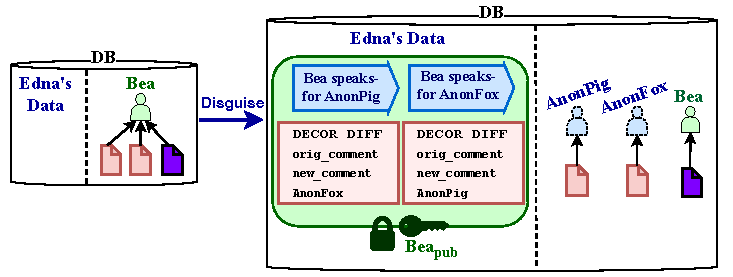
\includegraphics{figs/lobsters_catanon_visual}
    \caption[Topic-based anonymization creates pseudoprincipals and
    disguise records.]{When \sys applies topic-based anonymization to Bea's comments on
    stories tagged ``Star Wars'' (red), these comments are decorrelated to
    pseudoprincipals (``AnonPig'', ``AnonFox''). \sys stores encrypted
    speaks-for records mapping Bea to their
    pseudoprincipals, and diff records containing the comments with
    modified foreign keys.}
\label{f:lobsters_visual}
\end{figure}


%
To perform Bea's topic-based anonymization (Figure~\ref{f:lobsters_visual}),
which allows Bea to hide their association with a particular category of
content,
%
\sys thus:
%
\one{} queries the database to fetch comments and votes by Bea
affiliated with ``Star Wars'';
%
\two{} creates a pseudoprincipal (\eg
``AnonFox'') for every ``Star Wars''-tagged story that Bea commented
on, and inserts it as a new user;
% into the database;
%
\three{} modifies the database by rewriting comment
foreign keys to point to the created pseudoprincipals, and
removing Bea's votes on those stories;
%
\four{} creates new speaks-for records that map Bea to the created
pseudoprincipals and add links to Bea's speaks-for chain; diff records
containing Bea's votes on ``Star Wars'' stories; and diff records that document
Bea's original ownership of ``Star Wars''-tagged comments and the placeholder
pseudoprincipal data;
%
\five{} encrypts the speaks-for and diff records with Bea's public key and stores
them; and
%
\six{} returns a unique \xx ID to the application.

%
% \sys's security properties require that \xx records be untraceable: even a
% complete dump of \sys's state should not allow an attacker to match \xx records
% with users.
% %
% But efficient revealing requires there be a way to reference the records for a
% given \xx transformation and principal.
% %
% To this end, \sys encrypts both \xx records \emph{and} references to \xx
% records using principal public keys, which we describe next.
%
%We now describe how this works.
%

\sys adds a \emph{\xx table} and a \emph{principal table} to the application
database to store principals' \xxed data.
%
The \xx table contains per-disguise, per-principal lists of diff and speaks-for
records encrypted with the principal's public key.
%(Recall that private keys are not stored in the database.)
%; for instance, \verb+\xx_table[1]+ might be a list of \xx records
%pertaining to Bea's \xxing of ``Star Wars'' comments.
%
%These records are encrypted
%by Bea's public key, and thus can only be decrypted when Bea's private key is
%available.
%

\begin{figure}
    \centering
    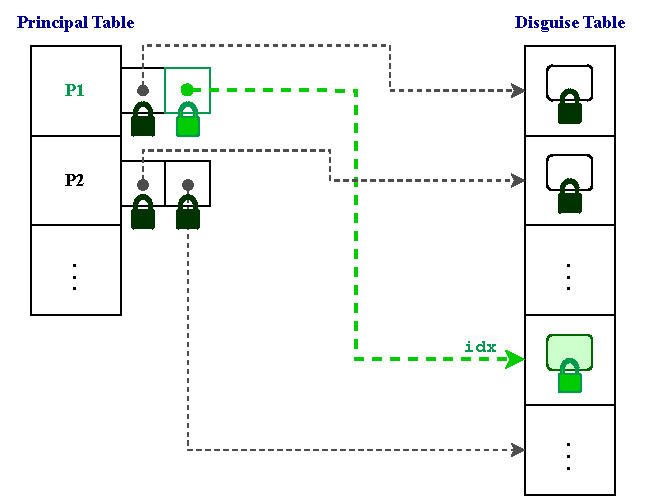
\includegraphics[width=.8\textwidth]{figs/indexes}
    \caption[\sys stores disguised data using a layer of indirection with
    encrypted indexes.]{When \sys applies a disguise to $P_1$'s data, diff
    records and speaks-for records for $P_1$ are stored at some random index
    \fn{idx} in the disguise table, and the encrypted index is appended to the
    principal table entry for $P_1$.}
\label{f:indexes}
\end{figure}

The principal table is indexed by application user ID; each row contains the
principal's public key, and a list of \xx table indexes encrypted with the
public key.
%
To store records for principal $p$ after some disguise, \sys \one{} encrypts the records with
$p$'s public key; \two{} stores the ciphertext in the \xx table under index
\fn{idx}; \three{} encrypts \fn{idx} (salted to
prevent rainbow table attacks) with $p$'s public key; and \four{} appends the
encrypted \fn{idx} to $p$'s list of encrypted \xx tables indexes
in the principal table.
%
Figure~\ref{f:indexes} shows how \sys adds a new disguise's diff records and
speaks-for records for $P_1$ to the disguise table at some index \fn{idx}; \fn{idx} is itself
encrypted and added to \sys's principal table for $P_1$.

%an encrypted $[i \parallel \text{random-nonce}]$ (encrypted with the principal's public key).
%encrypts $[i \parallel \text{random-nonce}]$ with the principal's public
%key and appends the result to its principal table record.

%
This allows \sys to store records without needing access to the principal's
private key, and to do so securely: the principal table adds a layer of
indirection from user ID to encrypted records, so an attacker cannot link
principals to their records.
%
At reveal time, \sys can efficiently find \xxed data for a given user
by decrypting and using \xx table indexes in the principal table.
%
%This also hides from an attacker which \xxed data belongs to a given principal
%because entries in the principal table cannot be interpreted without
%principals' private keys, which are not stored in the database.
%

%
\Xxing transformations may completely remove a principal from the
application database.
%
When this happens, \sys moves the corresponding list of encrypted \xx table
indexes from the principal table to a \emph{deleted principal table} indexed
opaquely, \eg by the public key.
%
This removes the user ID from the database while allowing future reveal
operations by the principal to find their \xx table indexes.
%
\sys also stores a special type of remove diff record that contains the
principal's ID and the principal's public key when a disguise removes a principal.  This
allows \sys to restore the principal to \sys's principal table if a user later
reveals the disguise.
%

%%%%%%%%%%%%%%%%%%%%%%%%%%%%%%%%%%%%%%%%%%%%%%%%%%%%%
\section{Revealing}
\label{s:reveal}

%
To apply a reveal transformation, \sys first locates and decrypts the
corresponding diff and speaks-for records using a \xx ID and the user’s reveal
credentials.
%

\begin{figure}[t]
  \small
\begin{lstlisting}[style=pseudo,escapeinside={(*}{*)}]
Reveal(disgID, uid, privkey):
 encrypted_disg_table_idxs := principal_table[uid]
 decrypted_disg_table_idxs :=
    decrypt(encrypted_disg_table_idxs, privkey)
 for idx in decrypted_disg_table_idxs:
   records = decrypt(disg_table[idx], privkey)
   for rec in records:
     if rec.disgID == disgID:
       // apply rec to application database
       // remove rec from disg_table
     else if rec.type == SPEAKS_FOR:
       // recursively reveal for pseudoprincipal
       // generated by another disguise
       Reveal(disgID, rec.pp_uid, rec.pp_privkey)
\end{lstlisting}
    \caption[Revealing restores all
    reachable disguised data using the user's reveal credentials.]{Pseudocode for revealing a \xxing transformation while
    application principal \fn{uid} exists. Recursive revealing (the
    \texttt{\small else} clause) walks the speaks-for chain to reveal composed
    records of pseudoprincipals created by other disguising transformations
    if necessary (\S\ref{s:composition}).}
  \label{f:revealpseudo}
\end{figure}

\texttt{RevealData} first derives the user's private key from their provided
reveal credentials, and invokes \sys's reveal procedure
(Figure~\ref{f:revealpseudo}) with this key. The procedure first looks up all
\xx records related to the provided reveal credentials via \sys's principal and
\xx tables.
%
\sys then applies diff records created for the \verb+disgID+ \xx transformation
to the database, thus restoring the relevant application objects to their
pre-\xxed state.
% Additionally, \sys recursively applies the procedure for
% pseudoprincipals that the current user speaks-for; this supports the
% composition of \xxing transformations, such as a Lobsters user who removes
% their previously-anonymized contributions (\S\ref{s:composition}).

%
To preserve referential integrity, \sys restores
\xxed data that was removed from tables in topologically-sorted order (constructing the dependency graph as in \S\ref{s:applying})
%
\sys then reveals any modifications, and finally performs recorrelations. 
%
In general, to reveal a diff record, \sys removes the placeholder row
and inserts the original row (both of which are recorded in the diff record).
%
However, for efficiency, \sys first checks if a placeholder row in diff records
has the same identifiers (\eg a primary key) as an original data row in the diff
record, and if so, updates the relevant columns of the placeholder row instead.
%

%
Finally, \sys de-registers any pseudoprincipal who no longer has any associated
disguised data, removing them from the principal table and the application's
users table.
%
Developers can configure \sys to also check for references to pseudoprincipals
prior to removing them, and depending on the application's needs, configure \sys
to delete, rewrite, or leave the references in place.
%
After revealing, the \xxed data is no longer needed, so \sys clears the
corresponding diff and speaks-for records.
%

%
In the example, if Bea wants to reveal their ``Star Wars'' contributions,
Lobsters invokes \sys with the \xx ID and Bea's password as reveal credentials.
%to reveal their Star Wars \xxing transformation.
%
\sys uses the password to reconstruct Bea's private key, retrieve and decrypt
Bea's records, and filter those records for those with the \xx ID.
%
\sys then restores deleted votes and Bea's ownership of
decorrelated comments.
%

\section{Global Database Updates}
\label{s:design:updates}
\sys's revealing as described thus far may reveal data that ignores
database updates applied since the time of disguise, such as global
transformations to un\xxed data or schema changes.
%
To prevent this, \sys utilizes reveal-time update specifications provided by the
developer to apply updates to \xxed data prior to revealing it. This ensures
that revealed data correctly reflects the current state of the database and any
implicit application-level invariants.
%
Prior to revealing the updated data, \sys also performs consistency checks
to guarantee adherence to internal database invariants, such as uniqueness
constraints.
%
Here, we describe how developers specify reveal-time updates; how \sys applies
these updates to data to reveal; and \sys's consistency checks.

%
\subsection{Global Data Transformations}
\label{s:design:dataupdates}

\begin{figure}
    \centering
    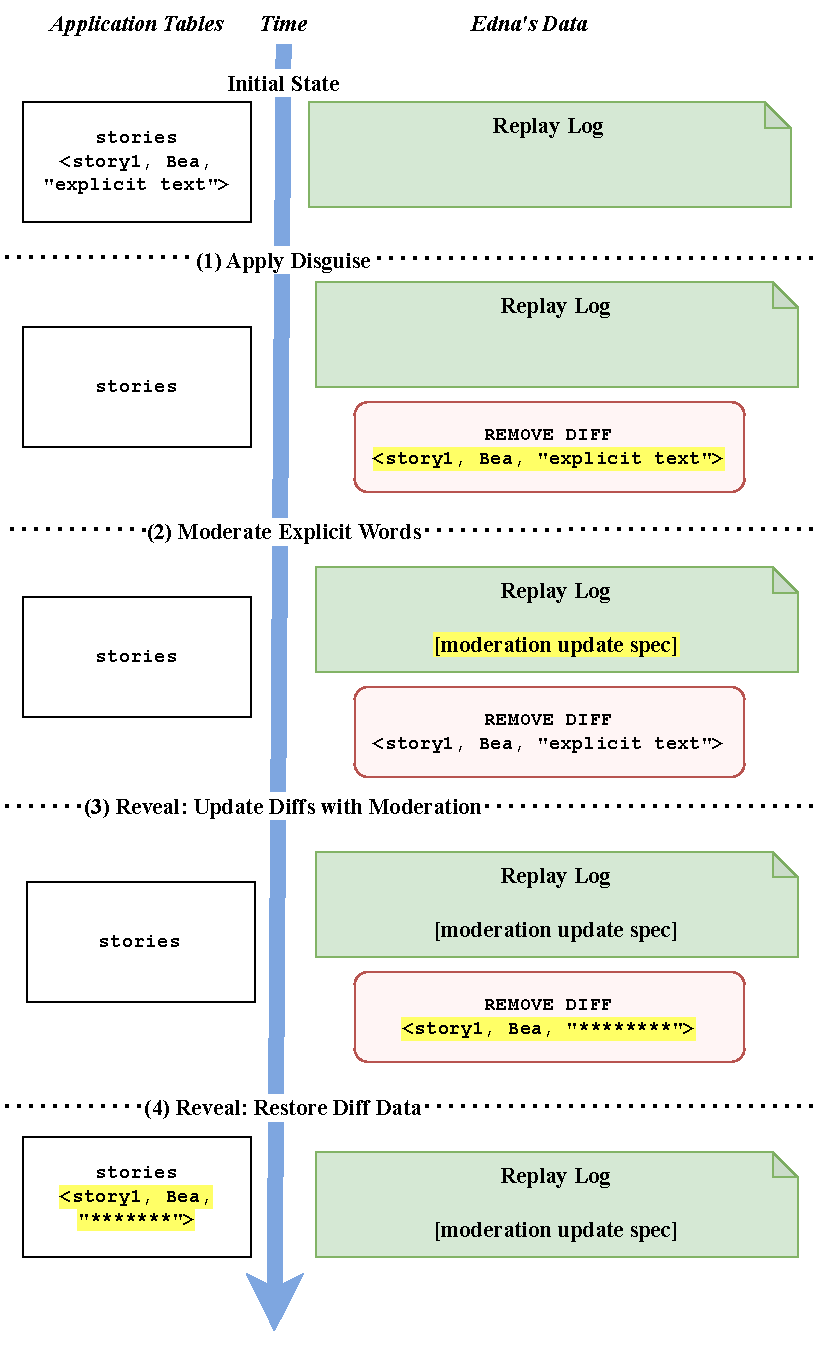
\includegraphics[width=.8\textwidth]{figs/update-moderation}
    \caption[During reveal, \sys applies reveal-time update specifications for
    global moderation updates.]{When the application applies updates like moderations of explicit
    words, it invokes \sys to log the corresponding reveal-time update specification. \sys then applies the
    update to disguised data in diff records prior to revealing them. Yellow 
    highlights changes to the application data or \sys's data.}
\label{f:update:mod}
\end{figure}
    
In order for revealing to preserve application correctness, \sys must obey 
global database updates that transform application data.
%
Consider an example: a moderator edits all posts to remove
swear words, creating an implicit invariant that all posts created prior to the
last moderation pass should contain no swear words.
%
If a user's disguise removes their posts, then a moderation pass occurs, and
then the user wants to restore their posts, \sys might incorrectly restore the
original post content with swear words present upon reveal.
%
However, \sys could correctly restore the post if it knew to remove the swear
words prior to reveal.
%
%Likewise, if \sys removed the post instead of scrubbing its content, the
%moderator would never see it (and could not edit it), but \sys would reveal the
%post with swear words still present.
%
%In the first scenario, \sys knows that an update was applied, and refuses to
%reveal the modified post; in the second, \sys does \emph{not} know that
%moderation happened and reveals the removed post.
%%
%Neither might be what the application desires.
%

%\sys handles this situation by tracking applied updates in a
%\emph{replay log} of update specifications.
%
Figure~\ref{f:update:mod} demonstrates how \sys applies updates to
disguised data using \sys's \emph{replay log} with \emph{reveal-time
update specifications}:
\begin{enumerate}[nosep]
    \item[(1)] \sys disguises some user data.
    \item[(2)] The developer invokes \sys with a reveal-time
        update specification when 
performing a global update that must hold over disguised data when it is
        revealed (\eg moderations). \sys records the update specification in its
        replay log. Update specifications map the original data and the
        placeholder data in diff records to corresponding updated-original and
        updated-placeholder data. 
    \item[(3)] When revealing data, \sys applies, in order, every specified
        update in the
        replay log added since the time of disguise to the disguise's diff
        records. In this case, \sys moderates explicit story text.
\item[(4)] After applying all updates to placeholder data, \sys reveals the
    updated rows in the diff record like normal.
\end{enumerate}
%
%Similarly, after applying all updates to the original data, \sys takes the
%updated-original data and restores it to the database.
%%
%As before for efficiency, \sys will first check if an updated-placeholder row has
%the same identifiers as an updated-original data row, and if so, will update the
%relevant columns of the placeholder row instead.
%
%
In the swear words moderation example, \sys queries the replay log, sees
the swear words moderation entry, and then applies the swear words moderation to
the removed post data in the diff record. Only then does \sys restore the post
with no swear words.\footnote{Note that in this example, the diff
record contains no placeholder data that replaced the removed post; in other
scenarios such as decorrelation or modification, \sys would apply the logged
update to diff placeholder data as well, in order to find the matching version in the
database and remove it.}

\subsection{Schema Changes}
\begin{figure}
    \centering
    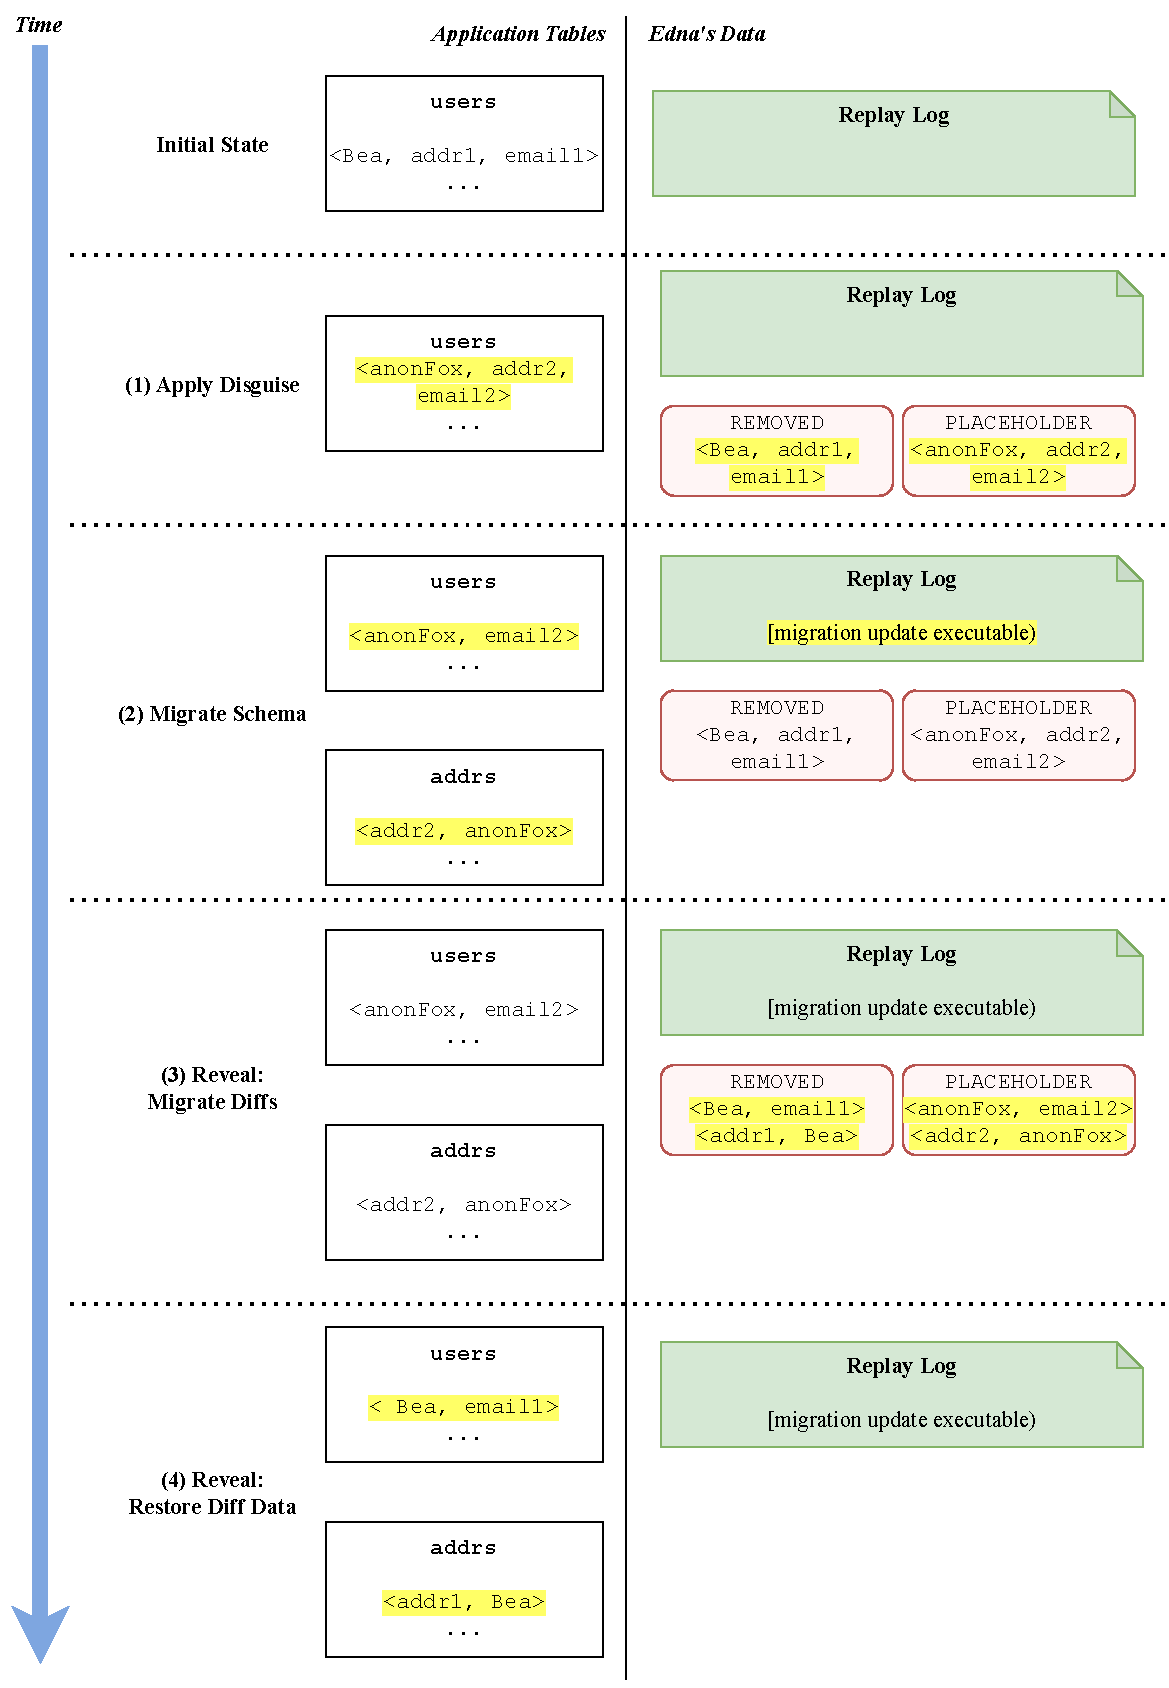
\includegraphics[width=.8\textwidth]{figs/update-migration}
    \caption[During reveal, \sys applies reveal-time update specifications for
    schema changes.]{Similar to a moderations update, the
    application notifies \sys of a schema change to apply to diff records
    prior to reveal. The schema change creates an address table with a foreign
    key to user rows, and removes the address from the user rows. This allows users to have multiple addresses.
    %
    Yellow highlights changes to the application data or \sys's
    data. For simplicity, the figure shows only the placeholder data of a pseudoprincipal row; in reality, placeholder data exists as part of \eg a decorrelation
    diff record.}
\label{f:update:schema}
\end{figure}

%
Applications also undergo database updates to migrate their schema in
order to reorganize data or add new application features. When these occur, \sys
must know how to manipulate any disguised data structured in the old database
layout to match that of the current database.
%
At first glance, schema changes might seem like a different class of
database update than global data transformations like content moderation, and
thus require a different approach.
%
However, the technique described in \S\ref{s:design:dataupdates} for global 
changes allows \sys to handle schema changes as well. 
%

%
Take, for example, a developer of an application with a \texttt{users} table
that contains rows with \texttt{username}s, \texttt{addr}s, and \texttt{email}s.
The developer may choose to allow users multiple addresses via a schema
change. To do so, they would create a new \texttt{addrs} table, with a
foreign key to the users table, and populate \texttt{addrs} using the address
data in \texttt{users}.  Finally, they would remove the \texttt{addr} column
from \texttt{users}.
%

Figure~\ref{f:update:mod} demonstrates how \sys applies such a schema change 
to disguised data.  \begin{enumerate}[nosep]
    \item[(1)] \sys disguises some user data.
    \item[(2)] The developer invokes \sys with a reveal-time update
        specification when 
performing the schema change; \sys records the update specification its replay log.
    \item[(3)] When revealing data, \sys applies the schema change update
        to diff record data, which maps an original \texttt{users} data row to
        both
    a row in \texttt{users} with username \texttt{uid} and a row in
\texttt{addrs} that has a foreign key of \texttt{uid} to \texttt{users}.
%
The update also generates two rows for any placeholder \texttt{users}
data row in a diff record.
%
\item[(4)] \sys then respectively restores and removes the migrated original data and placeholder
        data respectively, both of which now consist of one \texttt{users} and
        one \texttt{addrs} row.
\end{enumerate}

\subsection{Consistency Checks for Internal Invariants} 
After applying any developer-specified reveal-time updates that occurred since
the time of disguising, \sys performs consistency checks on the data to reveal
to ensure that revealing will not violate the database's integrity.
%
These checks allow revealing only if the revealed data: \one{} will still
satisfy uniqueness and primary key constraints; \two{} will not overwrite
updates that occurred while data was \xxed; and \three{} will maintain
referential integrity.

For \one{}, \sys checks that \emph{removed} \xxed data is still removed from the
database.
%

%
For \two{}, \sys ensures that \emph{modified} \xxed data is in the same modified
state and \emph{decorrelated} \xxed data is still affiliated with the same
pseudoprincipal in the database using the new value stored in the diff record.
%
\sys performs checks at column granularity. For example, a disguised
row can have two modified columns, but at the time of reveal, \sys finds that
only one column value remains at the modified disguised state that \sys expects.
The application thus must have updated the other column value since the time of
the disguise. \sys will only reveal the one column that matches the value \sys
disguised it to, in order to avoid overwriting application database updates.
This results in a partial restoration of the disguised row. Developers can
set argument \texttt{allow\_partial\_row\_reveals = false} when invoking
\texttt{RevealData}, which prevents \sys from revealing some disguised
columns of a row, but not others. With this flag set to false, if the the application had changed \emph{one} disguised column value
since the time of disguise,
then \sys will not reveal \emph{any} disguised column in the
row .
%

%
To ensure \three{}, \sys checks for the existence of all objects referenced by
the data to reveal (\eg a post referenced by a to-be-revealed comment).
%and ensures that any foreign key references to pseudoprincipals to be deleted
%are rewritten to the original.

\sys is conservative and will never reveal rows for which checks fail; the
affected data remains \xxed.  For example, if a developer chooses not to
register conflicting global database updates, \sys's checks may
fail, preventing disguised data from being revealed.
%
\sys could log encountered conflicts, giving the application a chance to fix
them so a later reveal can pass the checks.


%%%%%%%%%%%%%%%%%%%%%%%%%%%%%%%%%%%%%%%%%%%%%%%%%%%%%%%%%%%%%%%%%
\section{Shared Data}
\label{s:design:shared}

\begin{figure}
    \centering
    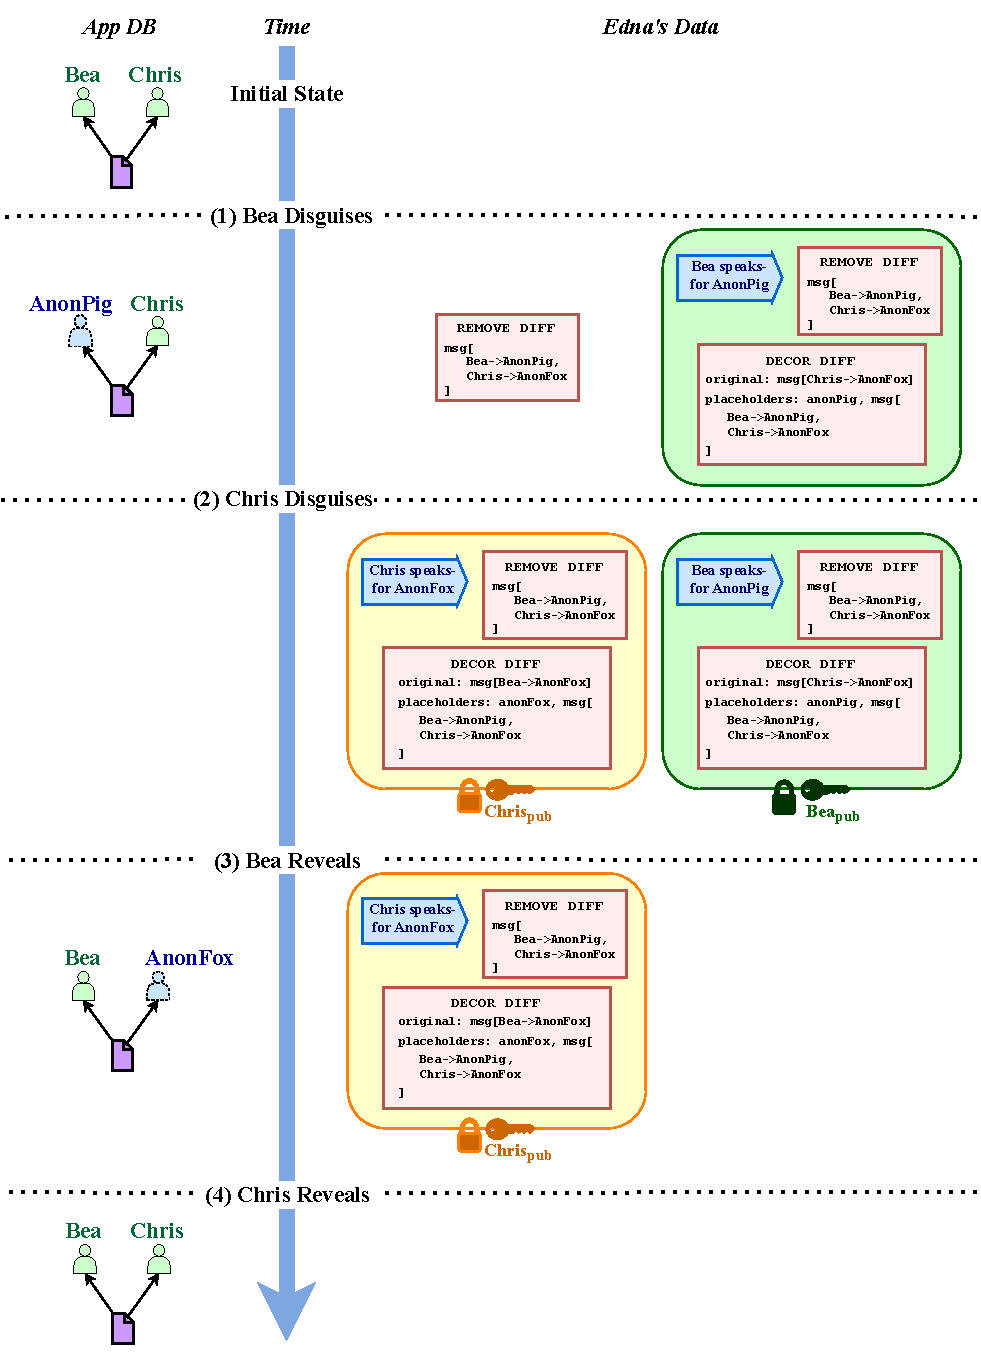
\includegraphics[width=\textwidth]{figs/shared_data}
    \caption[\sys implements disguising of shared data using
    pseudoprincipals and diff records.]{(1) When Bea removes their message, \sys
    creates and stores a fully-decorrelated diff record of the message
    (modifications to the shared message data are depicted using
    [owner$\to$pseudoprincipal] notation). Bea's disguised data also stores a
    speaks-for record to AnonPig.
    %
    (2) When Chris later removes their message, \sys stores a fully-decorrelated
    diff record in Chris' disguised data and a speaks-for record to AnonFox.
    \sys also deletes the message from the database, since it has no referencing
    users
    %
    (3) When one user (\eg Bea) reveals, \sys restores the
    fully-decorrelated message and recorrelates Bea with it.
    %
    (4) When Chris later reveals, they find the message already restored and
    simply recorrelate with their pseudoprincipal, AnonFox.
    }
\label{f:shared:data}
\end{figure}

\sys supports joint ownership semantics for shared data by modifying its design for
removal when encountering a shared object.
%
The first time any owner removes the data, \sys would normally remove the data
object. However, since the other owners have not since removed the data, \sys
must keep the data object around, but dissociated from the removing owner.
%

%
\sys ensures that \one{} if any user removes the data, then the data is
decorrelated from their identity; \two{} if all users have removed the data, the
data is removed from the database; and \three{} if any user returns, the data is
restored to the database with only revealed users recorrelated.  
%

%
To support these semantics, \sys creates a \emph{partially-removed} metadata
table. The table is indexed by a data row's unique identifier columns (\eg a
primary key id); each index maps to a (plaintext) remove diff record for a
shared data object. The diff record contains the shared data row, but where the
row has been fully\-decorrelated: all foreign keys to owners of the object have
been rewritten to refer to a pseudoprincipal.
%
Entries in the partially-removed table ensure that all owners agree on the
partially-removed state of shared data (\eg when some users are gone but others
remain, so pseudoprincipals replace the removed users). This allows users to
reveal consistently no matter which user reveals the shared data object first. 
%


Figure~\ref{f:shared:data} depicts how \sys executes over shared
data:
%
\begin{enumerate}
    \item[(1)] When any owner removes some shared data row, \sys checks the
        partially-removed metadata table with the data's identifiers.
        
        If \sys does \emph{not} find a matching entry, as in
        Figure~\ref{f:shared:data}, then \sys creates a fully-decorrelated
        version of the data row (with all foreign keys to owner replaced with
        random pseudoprincipal identifiers). \sys then inserts this into the
        partially-removed table.

        A matching entry must now exist; \sys takes the matching entry and
        stores a copy of the entry's fully-decorrelated diff record for the
        disguise.  As shown in step 3, this information will let an owner
        restore the data to the database if all owners have removed, and the
        data no longer exists in the database.  Importantly, every owner's diff
        record of the shared data will only reference another owner's
        \emph{pseudoprincipal} instead of their true identifier.

        \sys then creates the pseudoprincipal that matches the corresponding
        decorrelated foreign key to the owner, and stores diff records recording
        the pseudoprincipal row and foreign key rewrite for the owner. Finally,
        \sys stores a speaks-for record recording which pseudoprincipal the
        owner can speak-for. These records allow the owner to recorrelate back
        with the shared data after the data is restored to the database in a
        decorrelated state (steps 3 and 4).

\item[(2)]
        When the last remaining owner removes the data (all other owners are
        pseudoprincipals, \ie all other owners have removed the data), \sys
        removes the shared data row from the application database, and the
        corresponding entry from \sys's partially-removed table.
%

\item[(3)]
When \emph{any} owner chooses to return, \sys first restores the
fully-decorrelated row to the database as well as the partially-removed table,
        using the copy of the fully-decorrelated diff record in
the owner's disguised data.  \sys then rewrites the foreign key for the
pseudoprincipal who currently owns the shared data to recorrelate with the
owner, and removes that pseudoprincipal, revealing the other diff records like
normal. 
%

\item[(4)] If a subsequent owner reveals the shared data, \sys's consistency
    checks will prevent the reveal of the fully-decorrelated row (inserting the
        row will cause a duplicate row in the table). However, \sys will still
        rewrite the foreign key for that owner's pseudoprincipal to the original
        owner, and remove the pseudoprincipal from the database, thus
        recorrelating the data to the owner and restoring ownership.
%
\end{enumerate}

Note that the partially-removed table entry for any shared data object is
created only once: the first time any owner's disguise removes the shared data
object. Future removes after reveals will reuse the same partially-removed table
entry.
%
\sys thus ensures that any user who reveals and then removes the shared data
again decorrelates to the \emph{same} pseudoprincipal as before.

%
With this design, \sys can disguise and reveal shared data no matter the order
in which its owners decide to remove or reveal it. If an owner never removes the
shared data, they will continue to be correlated and have access to the data
even if other owners remove it (and become pseudoprincipals); similarly, if an
owner never restores the shared data, the data will remain forever owned by the
owner's pseudoprincipal if other owners choose to restore it.
%

%%%%%%%%%%%%%%%%%%%%%%%%%%%%%%%%%%%%%%%%%%%%%%%%%%%%%%%%%%%%%%%%%

%%%%%%%%%%%%%%%%%%%%%%%%%%%%%%%%%%%%%%%%%%%%%%%%%%%%%%%%%%%%%%
\section{Composing \Xxing Transformations}
\label{s:composition}

\begin{comment}
\begin{figure}[h]
    \centering
    \small
    \begin{tabular}{c|c|c|c} %|m{0.08\linewidth}}
        Operation & Remove & Modify & Decorrelate \\
        \hline
        Remove & $\varnothing$ & $\varnothing$ & $\varnothing$\\ 
        \hline
        Modify & Remove data & Modify data & Decorrelate data\\ 
        \hline
        Decorrelate & Remove data$^*$ & Modify data$^*$ & Recursively decorrelate data$^*$\\ 
    \end{tabular}
    \caption{What happens when disguise operations compose, with the first
    operation on the vertical, and the second operation on the horizontal. $^*$
    represents operations that require special handling, using the user's reveal
    credentials to find previously-decorrelated data to disguise and recursively
    disguise them.}
    \label{tab:composition}
\end{figure}
\end{comment}

\sys supports composition of \xxing transformations, which occurs when a
transformation applies to data that \sys has previously \xxed in
some other way.
%
Reasoning about composition of transformations can be broken down to reasoning
about the composition of primitive operation pairs, \eg remove after
modify, or remove after decorrelation.
%

%
Many pairs result in trivial composition: no operation can be composed after a
remove (the data is gone), and any operation after a modify updates the
data as expected. 
%
However, operations after decorrelation result in more complex composition scenarios.
%
For instance, decorrelation after decorrelation could occur if a user
decorrelates some posts, after which an administrator decorrelates \emph{all}
posts. In this scenario, the administrator's \xxing operation applies to
pseudoprincipal-owned posts in the same way as it does to unmodified posts. This
creates pseudoprincipals that can speak-for other pseudoprincipals.  This notion
of chaining together pseudoprincipals creates \sys's \emph{speaks-for chains}.
\sys uses the pseudoprincipal's registered public key to encrypt pseudoprincipal
diff and speaks-for records, so \sys does not need to know its link to an
original principal in order to encrypt and \xx its data.
%

%
%For instance, a user could decorrelate their posts, after which an
%administrator could modify all posts (including those of pseudoprincipals) by
%removing associated metadata.
%

%Another interesting case is when a transformation should apply to data that a
%user owned, but that has already been decorrelated.
Removal or modification after decorrelation also require special handling. For
instance, a Lobsters user might first decorrelate some of their comments and
then request to delete all their comments (\eg by deleting their account).
%
But the decorrelated comments are no
longer linked to the original user; how can the deletion transformation find
them?
%
\begin{comment}
%\sys by default handles \xxing of previously modified or decorrelated data
%without any problems: pseudoprincipals have affiliated public keys, and \sys
%treats them the same as any other principal when \eg an administrator wants to
%\xx all users' posts.
%
%Users can reveal \xxed data on behalf of their pseudoprincipals as described in
%\S\ref{s:reveal}.
\end{comment}
%
\sys addresses this question by accepting optional reveal credentials as part of
the \xx operation.
%
Reveal credentials let \sys recursively decrypt speaks-for records and
create a speaks-for chain starting from the disguising user, represented
by speaks-for relationships between pseudoprincipals. \sys can then disguise all
data of all pseudoprincipals included in the speaks-for chain.
%

With reveal credentials, \sys decrypts the user's previous diff and speaks-for
records. Each speaks-for record includes the identifier for one of the user's
pseudoprincipal and the pseudoprincipal's private key, and creates a ``link'' in
the speaks-for chain. A pseudoprincipal's identifier allows \sys to find data
referencing that pseudoprincipal and apply \xxing transformations on behalf of
the this pseudoprincipal as well as the user. 
%
A pseudoprincipal's private key---its reveal credential---allows \sys to
recursively decrypt its speaks-for records, and disguise any pseudoprincipals of
this pseudoprincipal created by multiple decorrelations.
%

%When decrypting a 
%\sys uses pseudoprincipal private keys in decrypted speaks-for records as
%credentials to recursively find pseudoprincipals from multiple decorrelations.

%
%\begin{comment}
%This lets \sys support Lobsters users first decorrelating their data, and then
%removing (or modifying) it via an additional \xxing transformations applied
%with their reveal credentials.
%\end{comment}
%\lyt{Without reveal credentials, \sys would not \xx any of the
%user's data previously decorrelated to pseudoprincipals.}
%and include them in the query to the application database.
%

\paragraph{Out-of-Order Reveals.}
\label{s:design:oooreveals}

\begin{figure}
\centering
    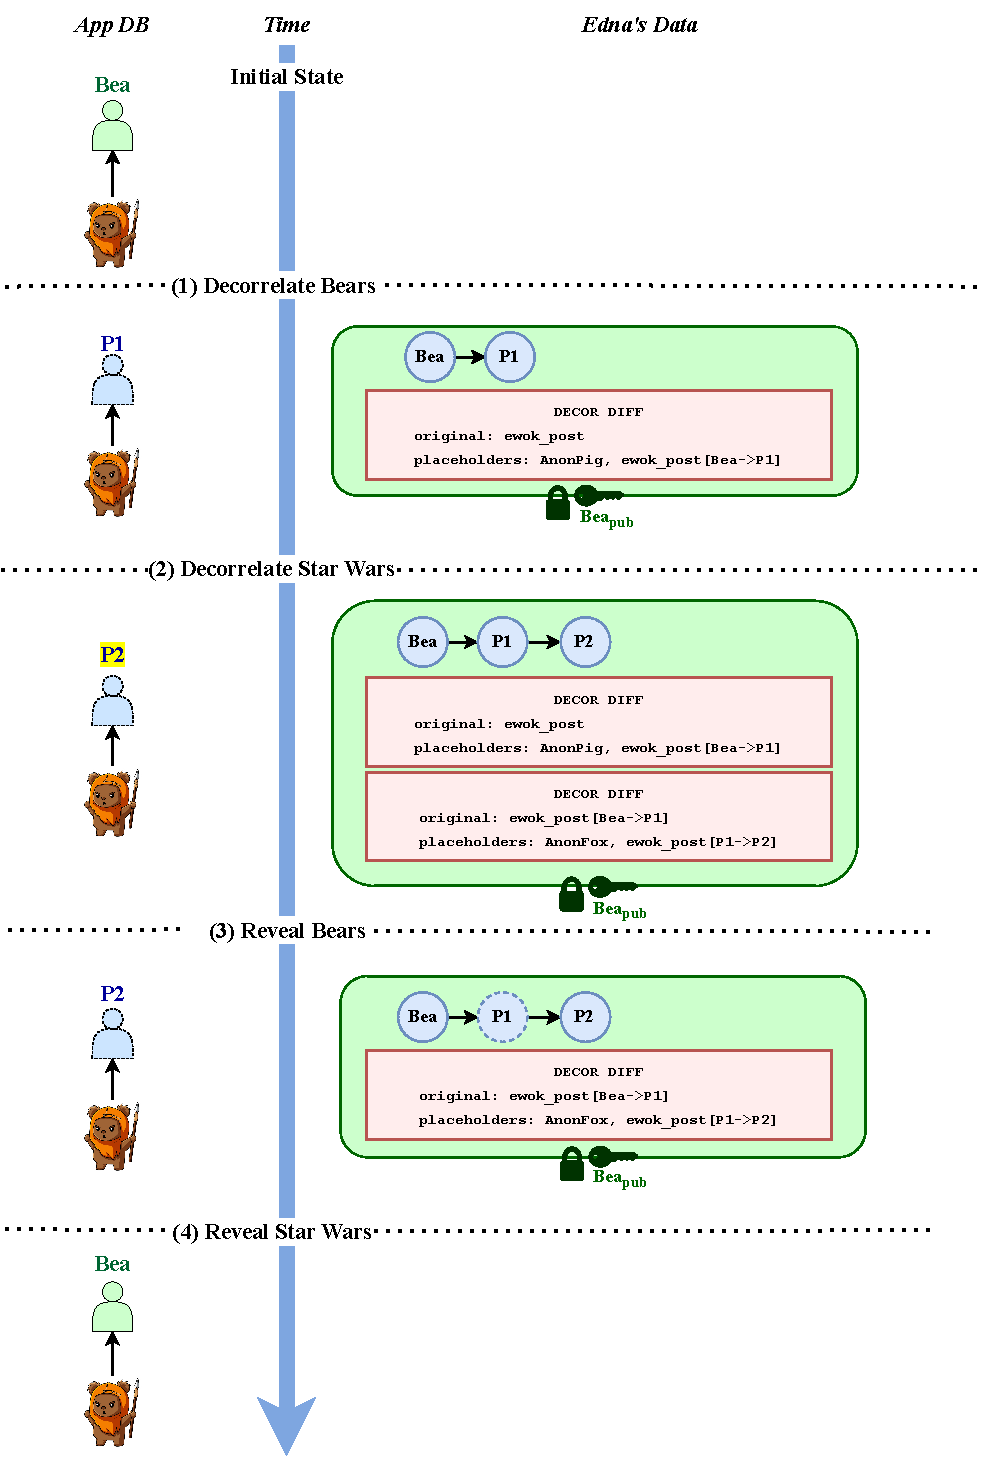
\includegraphics[width=0.83\textwidth]{figs/composition}
    \caption[Decorrelations can compose and be revealed in any order.]
    {\sys allows multiple decorrelations to compose, and can reveal them in
    any order such that the data remains decorrelated until the user reveals \emph{all}
    applied decorrelations. The speaks-for chain encoded in
    speaks-for records (shown in blue) allows \sys to handle recorrelation of intermediate
    pseudoprincipals. When Bea requests reveal of their ``Star Wars''
    posts (4) after revealing ``bears'' posts (3), \sys walks the speaks-for chain
    backwards from $P_2$ to find the latest principal that can speak-for $P_2$
    and has not yet been recorrelated. Thus, \sys restores ownership back to
    Bea.}
\label{f:composition-desn}
\end{figure}


\sys must also handle reveals of transformations in any order.  As before,
many scenarios are straightforward: revealing removals is trivial (data can
only be removed and restored once), and revealing modified data simply restores
the original (subject to consistency checks).
%
Handling out-of-order reveals of multiple decorrelations presents the greatest
challenge.
%
\sys's semantics (\S\ref{s:semantics:hl}) require that data that is decorrelated
multiple times will not be recorrelated until all \xxs are removed.
%also enables another desirable form of
%\xxing composition: .
%One desirable form of \xxing composition required special support:
%
For example, as shown in Figure~\ref{f:composition-desn} (left-hand side), if Bea
separately decorrelates their comments on ``bears'' and ``Star Wars'' posts,
then later reveals the ``bears'' posts, they might want Ewok-related comments
(tagged both ``Star Wars'' and ``bears'') to remain \xxed, even though they were
initially \xxed under the ``bears'' transformation.
%
%To realize this, \sys lets a \xxing transformation recursively operate over
%pseudoprincipals' data when their \emph{owner} (authorized through credentials
%that let them access a speaks-for record) invokes it.
%
%With reveal credentials, \sys finds pseudoprincipals with
%already-decorrelated comments and applies the \xxing transformation to these
%pseudoprincipals. This again creates pseudoprincipals that can speak-for other
%pseudoprincipals.
%
To support this, \sys again uses the speaks-for chain (\S\ref{s:composition}) that represent
speaks-for relationships between pseudoprincipals stemming from the revealing
user.
%
All reveal operations walk the full speaks-for chain to reveal all necessary
records (cf.\ Figure~\ref{f:revealpseudo}).

Furthermore, if reveal operations perform recorrelations out of order, \sys
removes an intermediate link in the speaks-for chain.
%
To describe how this works, take the example of two disguises that decorrelate
comments on ``bears'' and ``Star Wars'' posts respectively
(Figure~\ref{f:composition-desn}). 

%
\begin{enumerate}
    \item[(1)] First, the ``bears''
decorrelation rewrites Ewok posts to pseudoprincipal $P_1$.
%
\item[(2)] Next, the ``Star
Wars'' decorrelation composed on top decorrelates Ewok posts from $P_1$ to
pseudoprincipal $P_2$.  At this point, \sys has speaks-for records for Bea that
encode a speaks-for chain from Bea $\to P_1 \to P_2$.
%
\item[(3)] If Bea first reveals the ``bears'' anonymization---the first applied
disguise---on their data, \sys finds all accessible speaks-for records given
Bea's reveal credentials (cf.\ Figure~\ref{f:revealpseudo}), and constructs Bea's
speaks-for chain as a graph of principal-to-principal edges (namely Bea$\to
P_1\to P_2$).
%
\sys finds that $P_1$'s ``Ewok'' posts no longer exist in the database (they belong to
$P_2$ due to the composed ``Star Wars'' disguise), and thus does not restore 
``Ewok'' posts to Bea. \sys does still remove pseudoprincipal $P_1$ in the process
of restoring ``bear'' diff records, and once done, clears all ``bear'' 'diff
records from its encrypted disguise table. 
%
Importantly, however, \sys still retains the speaks-for record for Bea$\to P_1$,
since $P_1$ still has associated disguised data (namely a speaks-for record to $P_2$)!
%
\item[(4)] Now, if Bea reveals the second applied disguise---``Star Wars''---\sys finds
diff records for decorrelated ``Ewok'' posts whose original rows have $P_1$ as
owner. 
%
However, \sys cannot reveal the diff record directly and restore the
        decorrelated posts to $P_1$, as this will fail referential integrity
        consistency checks. Furthermore, the reveal of ``Star Wars'' reveals the
        last disguise applying to Bea's posts, so \sys should restore posts to
        their original, undisguised state (instead of decorrelated to $P_1$).


        Instead of immediately revealing the diff record, \sys walks the
        speaks-for chain (Bea$\to P_1 \to P_2$) backwards from $P_2$ to
        determine the \emph{next valid} principal in the chain who speaks-for $P_2$,
        which in this case is Bea.
        %
        A valid principal can either be a natural principal or a pseudoprincipal
        yet to be recorrelated. If a pseudoprincipal appears as placeholder data
        in any diff record of Bea's disguised data (from any disguise), \sys
        knows that it has not yet revealed that pseudoprincipal. Had \sys
        revealed that pseudoprincipal, then \sys would have removed its
        corresponding diff
        record.
        %

%
After determining that Bea is the next valid user in the speaks-for chain to $P_2$,
\sys rewrites the removed ``Ewok'' row in the diff record so that it references Bea instead of $P_1$,
and then restores the rewritten row to the database.
%
Finally, \sys deletes the diff records for the ``Star Wars'' disguise, the
speaks-for records for $P_2$ (which no longer has any associated disguised
data), and the speaks-for records for $P_1$ (which also has no associated
disguised data after $P_2$ is removed).
%
This implicitly truncates the speaks-for chain to simply be Bea.
\end{enumerate}
%
%This design works even in the presence of multiple recursive decorrelations and
%many-link speaks-for chains. 
\sys enforces the invariant that the chain only truncates at link
$L$ once all pseudoprincipals recursively generated in the chain beyond $L$ have
been recorrelated.
%

%%%%%%%%%%%%%%%%%%%%%%%%%%%%%%%%%%%%%%%%%%%%%%%%%%%%%%%%%%%%%%%%%%%%%%%%

%
%(in which case,
%an earlier link in the speaks-for chain may be removed).
%Pseudoprincipal-to-pseudoprincipal speaks-for relationships requires special
%handling during reveal operations: \sys %which must ensure that chains of speaks-for records remain linked to the
%original user even if reveal operations are applied out of order.

\begin{comment}

    To prevent such revealing behaviors, the user must provide their reveal
    credentials to tell \sys which pseudoprincipals the user can speak-for and
    whose data the user can recursively \xx.
%
    If Lobsters requires Bea to provide their reveal credentials when \xxing
    ``sci-fi'', \sys can then use those credentials to get Bea's speaks-for
    records, which relate Bea to any pseudoprincipal created for their ``Star
    Wars'' content.
%
    Equipped with the knowledge of these pseudoprincipals, \sys can now find
    comments that have the ``sci-fi'' tag \emph{even if} they also have the
    ``Star Wars'' tag (and thus have been already decorrelated).
%
    \sys then recursively decorrelates these dually-tagged comments from Bea's
    existing pseudoprincipals.
    %Rather than create a speaks-for record from \emph{Bea} to a new
    %pseudoprincipal , for these comments, \sys creates speaks-for records from
    %$p$ to $q$.
%

%
    Recursive decorrelation creates a chain of speaks-for records in \sys that
    ensures correct behavior on revealing.
%
    If Bea reveals their ``sci-fi'' comments first, the comments simply revert
    to being owned by Bea's pseudoprincipals.
%
    If Bea reveals their ``Star Wars'' comments first, \sys detects that
    dually-tagged comments are associated with another layer of pseudoprincipals
    in the application database, and does not reassociate them; instead, \sys
    simply
    %since the ``sci-fi'' \xxing transformation decorrelated the comment yet
    %again.
%
    %Comments with both tags continue to be owned by $q$, because \sys's reveal
    %process leaves modifications to the application database in place if they
    %happened after \sys applied the transformation it is currently revealing.
%
    internally updates the chain of speaks-for records so that only one layer of
    pseudoprincipals remain.

%
%
    %If Bea chooses to reveal the second transformation, \sys in both cases
    %reveals the original content, without having incorrectly revealed
    %``sci-fi'' comments in the intermediate state.
%
    %This composition is not a concern for votes, since the ``Star Wars''
    %\xxing transformation already removed them from application database.
%

%Lobsters expects that all ``sci-fi'' content decorrelated via category-based
%anonymization will remain decorrelated until Bea

\iffalse
% OUTLINE
% - introduce how pseudoprincipals are dealt with in the system
%    - have own keypair that is encrypted (chaining works)
%    - can own bags
%    - (encrypted) locators are kept as part of metadata for pseudoprincipald
% - process of chaining two \xxings
%       - go over steps in diagram (using example)
% - process of shared data
%       - use example of private messages here
An application may let a principal apply multiple \xxing transformations, some
of which may \xx data decorrelated to pseudoprincipals by some prior
transformation.
%
If data decorrelated by \xxing transformation $s$ could never be \xxed again,
then re-correlating the data by revealing $s$ might prematurely reveal data
\xxed by transformations applied after $s$.
%

\head{Composing Decorrelations.}
%
To solve this, \sys lets users \xx the data of pseudoprincipals that they can
speak-for.
%
This introduces a layer of indirection, so that revealing either transformation
will leave the decorrelating effects of the other in place.
%
To realize this indirection, \sys lets a \xxing transformation recursively
operate over pseudoprincipals' data when their \emph{owner} (authorized
through credentials that let them access a speaks-for record) invokes it.
%

%
In the example, \sys has access to Bea's reveal credentials when applying the
second \xxing transformation, so \sys can use those credentials to inspect any
of Bea's already-\xxed data.
%
This includes speaks-for records, which relate Bea to any pseudoprincipal $p$
created for their ``Star Wars'' content.
%
Equipped with the knowledge of these pseudoprincipals, \sys can now find
comments that have the ``sci-fi'' tag \emph{even if} they also have the ``Star
Wars'' tag (and thus have been already decorrelated).
%

%
Rather than create a speaks-for record from Bea to some new pseudoprincipal $q$
for these comments, \sys creates speaks-for records from $p$ to $q$.
%
This creates a chain of speaks-for records (Bea speaks-for $p$, which
speaks-for $q$) that ensures correct behavior on revealing.
%
If Bea reveals their ``sci-fi'' comments first, the comments simply revert to
being owned by $p$.
%
If Bea reveals their ``Star Wars'' comments first, \sys detects that these
comments are now owned by $q$ in the application database, since the ``sci-fi''
\xxing transformation changed the owner from $p$ to $q$.
%
Comments with both tags continue to be owned by $q$, because \sys's reveal
process leaves modifications to the application database in place if they
happened after \sys applied the transformation it is currently revealing.
%
\sys internally removes the mapping from Bea to $p$, and instead maps
Bea directly to $q$.
%
If Bea chooses to reveal the second transformation, \sys in both cases
reveals the original content, without having incorrectly revealed ``sci-fi''
comments in the intermediate state.
%

% --------------------------------------------------------------------------------

% Application of a new \xxing transformation $s_2$ on data \xxed
% by $s_1$ is relatively straightforward if $s_1$ only modified the data:
% %
% \sys encrypts stored records from $s_2$ with the associated principal’s public
% key, allowing that principal’s client to reveal the \xxing transformation by
% providing the corresponding private key. (\Xxing over data removed by $s_1$ is
% impossible because the data does not exist.)
% %
% However, if $s_1$ decorrelated data and reassociated it with pseudoprincipals,
% then $s_2$ cannot find the associated principal or its public key.
% %
% To solve this, \sys creates public/private keypairs for pseudoprincipals,
% encrypts pseudoprincipal data with pseudoprincipals' public keys, and lets a
% natural principal prove a speaks-for relationship with these pseudoprincipals.

% \lyt{Not sure if this is the right place...}
% In the following, we refer to all encrypted data that \sys produces when
% applying \xxing transformation $s$ as a \emph{bag}; locator \lcapa{ps} points
% to the bag of principal $p$'s \xxed data produced when applying $s$.

% %%%%%%%%%%%%%%%%%%%%%%%%%%%%%%%%%%%%%%%%%%%%%%%%%%%%%%%%%%
% \head{Storing Data for Pseudoprincipals.}
% %
% Each time \sys creates a new pseudoprincipal $q$ for natural principal $p$
% during $s_1$ (with $p$'s public key still available), it generates a keypair
% for $q$.
% %
% \sys then ``wraps'' $q$'s private key by encrypting it with $p$'s public key,
%  stores it with records created by $s_1$ at locator \lcapa{ps_1}, and
% forgets the plaintext private key.
% %stores it at bag pointed to by locator \lcapa{ps_1}, and
% %
% Hence, access to $q$'s private key---or records encrypted for $q$---requires $p$'s private key.
% %
% \sys then stores $q$'s public key via \fn{RegisterPrincipal} and uses it to encrypt $q$'s records.
% %
% This idea applies recursively: in the above example, $p$ itself may
% be a pseudoprincipal and not a natural principal.
% %
% (This is why the application cannot \eg simply email $q$'s private key to
% $p$ when it creates a pseudoprincipal $q$.)
% %
% In this case, \sys encrypts $q$'s private key with the public key of
% pseudoprincipal $p$, granting any natural principal who can access
% $p$'s private key access to $q$ and its data.
% %
% Thus, the bag at locator \lcapa{ps} contains both $p$'s encrypted records and
% pseudoprincipal private keys from \xxing transformation $s$.

% %%%%%%%%%%%%%%%%%%%%%%%%%%%%%%%%%%%%%%%%%%%%%%%%%%%%%%%%%%%
% \head{Pseudoprincipal Metadata.}
% %
% When $s_2$ creates a record bag encrypted for pseudoprincipal $q$, it produces
% locator \lcapa{qs_2} for the bag.
% %
% \sys stores this locator with pseudoprincipal $q$'s metadata, but encrypts
% it with $q$'s public key.
% %
% Encrypting pseudoprincipal locators ensures that \sys never exposes the mapping
% from a principal to its locators once a principal has \xxed their account (\sys
% returns all locators of natural principals to the application when \xxing, as
% described in \S\ref{s:design:\xxing}).
% %
% Locator \lcapa{qs_2} will only be needed to reveal $s_2$---and at that point,
% $q$'s private key will be available, as the principal who speaks-for $q$
% unwraps it.
% %

% %
% As an optimization, the application can tell \sys to return \lcapa{qs_2} instead
% of storing it; the application is then responsible to return the locator to
% the correct natural principal (\eg displaying a QR code to a client invoking $s_2$).
% %
% %$p$'s private key and bag locator \lcapa{ps_1} are available.
% %This causes \sys to return pseudoprincipal bag locators without
% This avoids an extra encryption per pseudoprincipal.
% %
% $p$ then reintroduces these locators when they reveal $s_2$.
% %

% \begin{figure}[t]
%     \centering
%     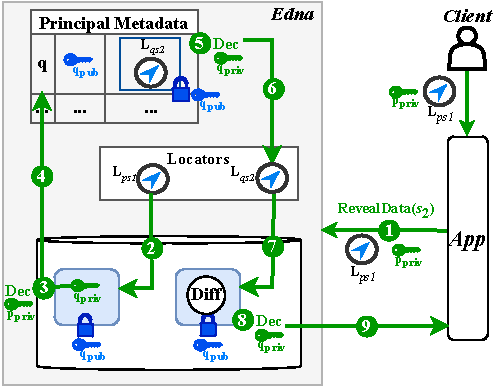
\includegraphics{figs/edna_reveal}
%     \caption{To retrieve diffs from composed \xxing transformation $s_2$, \sys
%              first decrypts $q$'s private key in $p$'s bag for $s_1$,
%              and uses that private key to decrypt \lcapa{qs_2} and the bag
%              it points to.}
%     \label{f:recursive}
% \end{figure}

% \newcommand*\circled[1]{\tikz[baseline=(char.base)]{
%             \node[shape=circle,draw,inner sep=1pt] (char) {#1};}}
% %
% Figure~\ref{f:recursive} shows how a natural principal reveals a composed
% \xxing transformation. %using the low-level API.
% %
% \lyt{(Added the following:)} In this example, clients provide private keys as reveal credentials.
% %
% \circled{1} The application asks \sys to reveal $s_2$ using $p$'s
% private key and \lcapa{ps_1}.
% %
% \circled{2}
% \sys looks up \lcapa{ps_1} to find $p$'s bag for $s_1$, and \circled{3}
% decrypts it with $p$'s private key.
% %
% This reveals that $s_1$ created pseudoprincipal $q$ and reveals $q$'s private
% key, so \circled{4} \sys looks up $q$'s metadata and
% \circled{5} decrypts $q$'s locators with $q$'s private key.
% %
% \circled{6} This provides \sys with \lcapa{qs_2}, so it \circled{7} looks
% up $q$'s bag for $s_2$, \circled{8} decrypts it with $q$'s private key,
% and finds the database diff applied for $q$ during $s_2$.
% %
% \circled{9} Finally, \sys reveals the \xxed data held in the diff,
% and returns to the application.
% %returns the diff to the application, which reveals the \xxing transformation.

% \head{Data Cleanup.}
% %
% When \sys reveals $s_1$ and recorrelates $p$ to its data, \sys removes both $q$
% and $q$'s public key from $q$'s metadata.
% %
% However, \sys must sometimes retain part of $q$'s metadata, as it may include
% encrypted locators that \sys must keep to later find $q$'s bags.
% %
% Given that \sys cannot decrypt $q$'s locators, nor send them to a client, \sys will still retain
% $q$'s metadata if the metadata contains encrypted locators after revealing.
% %when the application calls \fn{ForgetPrincipal} on $q$.
% %
% However, \sys marks $q$ as forgotten, so that \sys knows to delete $q$'s metadata when \sys clears
% all stored records at $q$'s locators during future \xxing transformation reveals.
% %

% %
% Because \sys may need to use \lcapa{ps_1} to access $q$'s encrypted private key, \sys retains $q$'s
% encrypted private key at \lcapa{ps_1} even if the rest of $s_1$'s \xxed data at
% \lcapa{ps_1} (\ie encrypted diff or speaks-for records) has been removed.
% %
% The bag is now empty except for $q$'s private key.
% %
% \lyt{Move to discussion?
% \sout{To hide that \sys deleted previously-stored data, it puts a random-length
% dummy record into the bag.}}
% %
% %Once \sys has removed $q$'s metadata, then \sys removes all trace of \lcapa{pd} since the
% %referenced bag is empty.
% %

% %
% %Natural principal $p$ fully reveals \xxing transformation $s_2$ by providing \lcapa{ps_1}: this locator must be
% %from the \xxing transformation $s_1$ that decorrelated $q$ from natural principal $p$.
% %
% To reveal $s_2$, \sys follows Figure~\ref{f:recursive} to find and reveal the
% records for $s_2$ at \lcapa{qs_2}. \sys also clears all records at \lcapa{qs_2}
% after revealing. Because $q$ has been marked forgotten, \sys then removes
% \lcapa{qs_2}, which points to a now-empty bag.
% %
% Once \sys has removed all metadata for $q$, \sys removes $q$'s private key and
% \lcapa{ps_1} since the bag is now empty.
%
\end{comment}


%%%%%%%%%%%%%%%%%%%%%%%%%%%%%%%%%%%%%%%%%%%%%%%%%%%%%%%%%%%%%%%%%

\section{Authenticating as Pseudoprincipals}

As described so far, if Bea wanted to modify a decorrelated ``Star Wars''
comment, they would have to reveal the comment, edit it using their normal
credentials, and then re\xx the comment again.
%
Applications that use \sys can also let users modify decorrelated records
without the reveal step via support from \sys's \texttt{CanSpeakFor} API call.
%
To support this, an application accepts reveal credentials along with a
modification request, and invokes \texttt{CanSpeakFor} with the credentials.
\sys uses these credentials to validate that the user speaks-for a specific
pseudoprincipal by walking the speaks-for chain (cf.\
Figure~\ref{f:revealpseudo}). This ensures that the user can access a speaks-for
record linked to the pseudoprincipal. After validating the user's request,
the application can proceed to 
update the database with the modification.
%
%previous diff records to reflect the newly modified state.
%

%%%%%%%%%%%%%%%%%%%%%%%%%%%%%%%%%%%%%%%%%%%%%%%%%%%%%%%%%%%%%%%%%
\section{Design Limitations}
\label{s:design:limits}

\paragraph{Disguises.}
\sys assumes that all desired disguises are captured with the three primitive
operations (remove, modify, and decorrelate).
%
Furthermore, disguising transformations may affect data processing of
application data (\eg aggregates over the number of users), or application side
effects dependent on application data (\eg sending notifications).  \sys
currently expects the developer to correctly handle these scenarios, and to ensure
that any modified aggregations or placeholder data do not violate application
correctness.
%

\paragraph{API.}
\sys's API assumes that:
\begin{enumerate}[nosep]
    \item the application uses a relational database;
    \item rows to \xx have direct foreign key relationships to a users table,
    where each user corresponds to a row of that table;
\item all rows to \xx are owned by (have a foreign-key relationship) to one or more principals; and
    \item all rows can be uniquely identified (\eg via primary key).
\end{enumerate}
%
Applications that fail to satisfy these assumptions---\eg because they have
complex ownership chains or use a NoSQL database---could be supported with
extensions to \sys's design. \sys could use techniques from DELF~\cite{delf} to
support multiple data models; 
%by requiring
%developers to provide \one{} a model of data as objects with dependency edges to other objects,
%and \two{} instantiations for update/delete/insert operations on these objects.
%
and K9DB's data ownership graph~\cite{k9db} to handle indirect data ownership.
If no user owns a data item, \sys could refuse to disguise it and flag the
developer to review the disguise specification.  
%
Finally, to address the unique identification requirement, \sys could add unique
IDs for every data object, so \sys can refind the object when revealing.
However, this method requires more invasive changes to application data. 
%

\paragraph{Shared Data.}
\sys's approach for shared data faces two main limitations. First, the
application cannot use foreign keys to the users table as unique identifiers for
a table's rows. \sys uses unique identifiers to determine which objects to
update upon a reveal, and also modifies foreign keys to the users table when
decorrelating and recorrelating users from a shared data object. Thus, if
foreign keys to the users table are modified, the unique identifier would change
as well, and \sys would incorrectly reveal shared data.
%
Note that this would not be an issue for a single-owner removal, since the
object is removed and not dissociated from the owner.
%
If foreign keys to users table act as unique identifiers, one potential solution
might introduce a layer of indirection by adding a new unique identifier (\eg an
autoincrementing primary key), at the cost of potential performance impacts.

Second, owners of shared data who remove and reveal the data multiple times 
decorrelate to the same pseudoprincipal each time. This may allow for more opportunity
for observers of the application to determine which pseudoprincipal corresponds
to which user (although this falls outside of \sys's threat model).
To see why \sys requires this limitation, imagine the following counterexample:
\begin{enumerate}
    \item[1)] Bea and Chris both remove a shared message, so no data is left in
        the database. Both Bea and Chris store a diff record of the message mapping Bea to $P_1$,
        and Chris to $P_2$. 
       
    \item[2)] Chris first reveals and then removes the message again, so no data
        is left in the database. Chris now stores a diff record of the message
        with Chris mapped some \emph{new} pseudoprincipal $P_3$.
        
    \item[3)] Now Bea reveals, restoring the message with $P_1$ and $P_2$ to
        the database. 
        
    \item[4)] Chris attempts to reveal the message, but cannot find $P_3$ in the
        database, and thus fails to recorrelate with the message. 
\end{enumerate}
%
Chris' reveal's failure arises because Chris and Bea disagree upon what
data---in particular, which pseudoprincipal references---to insert into the
database, should the shared data object no longer exist. Chris believes it to be
$P_3$, whereas Bea will restore to $P_2$ for Chris. 
%Chris and Bea must agree,
%because \emph{any} owner can perform the final removal of the data from the
%database, and \emph{any} owner can perform the first reveal that restores data
%back into the database.
To remedy this, \sys uses the partially-removed table to ensure that owners
agree on the intermediate states of partially removed data.
%


%TODO pseudoprincipal created upon disguise and not for all principals at once

\paragraph{Reveal-Time Updates.}
\label{s:design:updates:limitations}
%\sys's replay log also faces some limitations.
%
%First, developers must do additional work to add hooks to invoke \sys when any
%major application change or schema change occurs. 
%%
%Invoking these hooks and applying these updates during reveal also adds
%additional computation work; we measure these costs in \S\ref{s:eval:updates}.
%

%
Reveal-time updates in replay logs only apply to diff records, which contain the actual
data changes, and not speaks-for records; \sys assumes that the identifiers for
principals in speaks-for records that encode the speaks-for chain remain
consistent as the database changes, allowing \sys to use its composition
techniques with speaks-for chains (\S\ref{s:design:oooreveals}) to reveal
multiple disguises in any order.
%

%
Furthermore, as described in \S\ref{s:overview:updates}, \sys assumes that
any nondeterminism or update side effects will maintain application
correctness.
%
One potential extension would be for developers to indicate the data
dependencies of each update. To handle the unsupported example in
\S\ref{s:overview:updates}, \sys can use the knowledge that posts depend on
votes to restore disguised votes before posts. However, because votes have a
foreign key to posts, this requires \sys to disable foreign key checks and
carefully check for dangling votes that violate referential integrity after
restoring posts.
%, since restoring votes first can now inadvertently leave
%dangling pointers. 
%
A perhaps more realistic but more limited solution might require developers to
schedule periodic updates to ``fix up'' any rows that
have been revealed since the update. However, this only works for an idempotent
update, as it should not incorrectly update already-updated rows again.  
%

%%%%%%%%%%%%%%%%%%%%%%%%%%%%%%%%%%%%%%%%%%%%%%%%%%%%%%%%%%%%%%%%%

\section{Security Discussion}
\label{s:eval-security}


%
%We now analyze what security \sys's design provides.
%
\sys's design achieves confidentiality of disguised data between the time of
disguising and revealing, its key goal.
%
By contrast, some aspects of \sys's design help make \sys practical and
deployable without major application modifications, but give up stronger
security in exchange for usability.
%

%Because \sys encrypts \xxed data, \sys achieves:
%lyt: I didn't like this because we already talk about encrypting disguised data
%below, and this is only a subset of WHY Edna achieves these security guarantees
%
Under \sys's threat model, \sys achieves:
\begin{enumerate}[nosep]
    \item confidentiality of disguised data, via encrypting disguised data using asymmetric encryption, so only the owning user’s private key can reveal it;
    \item confidentiality of which encrypted disguised data belongs to which
        user, via opaque, encrypted indexing to reference a user’s disguised data; and
    \item reduced linkability between parts of a user's data, via splitting data ownership among pseudoprincipals.
\end{enumerate}
%
\sys provides decorrelation with pseudoprincipals to ease integration with
existing applications, even though pseudoprincipals (and their mere existence)
can reveal information to the attacker.
%
Pseudoprincipals preserve application data and referential integrity, ensuring
that \eg every post always has an author, or that vote counts on posts remain
unchanged, without requiring the developer to handle special cases of deleted
users and orphaned data.
%
However, this necessarily leaves information in the database: an attacker with
database access could see all application database content and code, and \sys's
\xx, principal, and deleted principal tables.
%
Thus, what the attacker learns includes:
\begin{enumerate}[nosep]
  \item any un\xxed data in the application database;
  \item the active principals that have \xxed data, via \sys's principal
      table;
  \item the pseudoprincipals currently registered, from \sys's
    principal table and the application DB;
  \item the number of deleted principals, via the size of the deleted
    principal table;
  \item the amount of \xxed data in \sys; and
  \item the \xx specifications, from application code.
\end{enumerate}

%

Leveraging the application database (as opposed to separate external storage) to
store \xxed data increases \sys's practicality because it avoids burdening users
with managing their disguised data.  However, this leaves potentially
exploitable metadata available to attackers.
%
An attacker could leverage pseudoprincipal groupings (\eg a pseudoprincipal
owning posts in both ``CMU 2018'' and ``BayArea'' topics), un\xxed data
(\eg comments signed with the user's name), and \sys metadata (\eg that some
anonymous user has more \xxed data than another, as \sys stores \xxed data without
padding for efficiency) to infer the identity of the original owning principal.

Finally, \sys makes no guarantees for users who actively use \xxed data after
compromise (\eg by revealing or editing decorrelated data): after an attacker
compromises the application at time $t$, they can harvest private keys that
clients provide after $t$.
%
However, \sys always protects users' \xxed data if they remain inactive.
%
%%Likewise, when a client provides $(\lcapa{pd}, p, d)$ to operate over data under
%%disguise, the attacker learns the correspondence between \lcapa{pd} and $(p, d)$.
%
%%But this merely makes the attack more efficient, as the attacker can already discover
%%$p$'s disguise history by attempting to decrypt all bags with $p$'s private key.
%
%However, the attacker cannot gain access to any previously-revealed data that users
%subsequently removed from the application database.
%

%
%: viable protections (\eg storing
%\xxed data externally, \xxing all user data, or padding \xx records and
%pseudoprincipal counts) can break application functionality by removing too much
%data, prevent further \xxing of pseudoprincipal-owned data, and result in
%prohibitively expensive space costs.
%

%
%The attacker could also try to leverage remaining data in the application
%database, the size of the \xxed data, and the number of registered
%pseudoprincipals for a statistical inference attack that lets them conclude
%which pseudoprincipals likely correspond to a natural principal.
%%
%\sys does not protect against such attacks: viable protections would break the
%application for others by removing too much data from the application DB and
%require expensive padding of \xxed data and the pseudoprincipal count.
%%

%as the cost of the necessary protections would be
%prohibitive: \sys would have to add padding to every bag and pseudoprincipal locator set, and the
%amount of padding would need to be proportional to the largest amount of data any natural principal
%holds in the application DB (see \S\ref{s:disc}).
%
%However, \sys guarantees that the attacker cannot tell the \emph{identity} of an inactive natural
%principal correlated with some pseudoprincipal(s) based on the compromised information, since the
%natural principal has been removed from the application DB and from \sys's metadata.


%We note that our threat model puts privilege-escalation and root privilege attacks out of scope:
%thus, an adversary cannot observe privilege-protected query logs or other database metadata that
%would potentially leak \xxed data~\cite{grubbs}. While \sys provides no guarantees for
%root-privilege attacks, \sys increases the difficulty of extracting \xxed data. \lyt{Move
%this last paragraph somewhere?}

%\textbf{Security of Reveal Credentials.}
%
%
The attacker never has access to a user's private key unless the user actively
provides their credentials.
%
The attacker also cannot access the private key of any pseudoprincipal because
\sys stores such keys in encrypted speaks-for records.
%
% By induction, the attacker cannot access any private keys.
%
If an application uses password-based reveal credentials, \sys
guarantees security equivalent to the security of the user's password.

\section{\sys without Encryption}
\label{s:noencrypt}

\iffalse
\begin{figure}[t]
\begin{lstlisting}[style=rust,escapeinside={(*}{*)}]
// disguises principal p according to the spec, 
// will disguise already-disguised data ((*\S\ref{s:composition}*))
(*\textbf{DisguiseData}*)(
        p: Option<UID>, 
        spec: DisguiseSpec,
        principal_gen: PrincipalGenerator,
        schema: Schema,
        disguise_over: bool) 
    -> disguiseID;

// Reveals data disguised by s for p with p's password. 
(*\textbf{RevealData}*)(
        p: UID, 
        pwd: Password,
        did: disguiseID, 
        pp_ref_policy: PseudoprincipalReferencePolicy,
        allow_partial_row_reveal: bool,
        schema: Schema)
    -> bool;

// Gets principals that p can speak-for.
(*\textbf{CanSpeakFor}*)(p: UID, pwd: Password) -> Vec<UID>;

// Applies an update spec to disguised data
(*\textbf{ApplyUpdate}*)(update_spec: UpdateSpec) -> bool;
\end{lstlisting}
\caption{Potential \sys API without Encryption of Disguised Data (Rust-like syntax).}
\label{f:newapi}
\end{figure}
\fi
%

Should developers want to support disguised data in a weaker threat model that
does not require encryption (as described in \S\ref{s:semantics:noencrypt}),
\sys still helps developers address the challenges of maintaining referential
integrity when a disguise is performed (creating pseudoprincipals as placeholder
users); composing disguises and reveals in arbitrary orders; disguising shared
data; and applying global updates to disguised data.
%
Furthermore, removal of encryption simplifies several aspects of \sys's design.
%
This section
describes these aspects and potential
alternative designs for disguised data without encryption. 

\paragraph{Design Simplifications.}
If \sys removes encryption of disguised data, disguised data remains accessible to
the application and updates can thus apply immediately to disguised data. \sys
therefore would not need a replay lot to help developers apply updates to
disguise data. 
%
Developers would still write update specifications corresponding to these
updates in order to update disguised data rows stored in the disguised tables.
%

%
Removal of encryption also eliminates the need for registration with a user
keypair, user reveal credentials, encryption/decryption on the disguise/reveal
paths, and encrypted indexes mapping a user to their disguised data. The
disguise table would hold plaintext disguised data, and \sys would not need the
principal table.
%

%
Furthermore, \sys can always disguise already-disguised data, since a user does
not need to provide a reveal credential in order to unlock their
already-disguised data. A developer instead can allow a user to specify whether
they wish to disguise their disguised data again using a boolean.
%

%
%This API still helps address the challenges of maintaining referential integrity
%when a disguise is performed (creating pseudoprincipals as placeholder users);
%composing disguises and reveals in arbitrary orders, and over shared data; and
%applying global updates to disguised data (albeit perhaps during update
%execution, rather than at reveal time).

%
\paragraph{Alternatives Designs Without Encryption.}
Instead of moving disguised data into a new database table for disguised data as
\sys does, developers could also choose to implement disguised data by logically
removing it using database flags and predicates (\eg \texttt{is\_deleted})
because disguised data need not be encrypted.
%
In this case, the developer must ensure that all queries for the data predicate
on the tag so the application does not return disguised data. Systems like
Qapla~\cite{qapla}---which this thesis compares to \sys in
\S\ref{s:eval-qapla}--- can help enforce these flag-based policies.
